%The main goal of the vertical jumper is (without much of a surprise) to jump as high as possible.
This example was designed to introduce \emph{bioptim}'s ability to reduce the number of degrees-of-freedom (DoF) of a model via the \texttt{mappings}, to account for nonlinear boundaries on the controls, and to solve complex multiphase programs including impacts and free time phases.

The model used was a full-body model consisting of 3~DoFs at the pelvis (forward and upward translations, tranverse rotation), 1~DoFs at each upper limb (shoulder flexion), and 3~DoFs at each lower limb (hip, knee and ankle flexion) for a total of 11 DoFs.
For this optimization, the \texttt{BidirectionalMapping} was used to symmetrize the left-hand side with the right-hand side, effectively creating a 7-DoFs pseudo-2D model. 
Since this is a full-body model, the root segment (i.e., the pelvis) was left uncontrolled, reducing the number of control variables to 4, namely the shoulder, hip, knee and ankle flexions. 

A total of five phases were used to describe the dynamics of the jump, flight and landing. 
The first two were push-off phases consisting in one phase with two ground contacts (heel and toe) and a second with one contact (toe). 
A contact is described as a point where forces are applied to cancel the acceleration. 
The third phase was purely aerial, described by a free-fall dynamics, i.e., without contact point.
The last two were landing phases, a first one with one contact (toe) and a second one with two contacts (heel and toe).
The transitions between phases with addition of contact points were approximated with the build-in inelastic impact \texttt{PhaseTransition.IMPACT}, which computes the velocity of the kinematic chain after an impact.

The main objective function was a Mayer objective computed at the end of the \comment{pushoff}{bizarre, tu utilises les équations paraboliques du free fall ?} phase consisting in maximizing the jumps height ($h$) such that:
\[
h = \frac{\dot{c_z^2}}{-2 g} + c_z,
\]
where $c_z$ and $\dot{c_z}$ are the center of mass position and velocity, respectively, and $g$ is the gravitional acceleration constant ($\SI{-9.81}{\meter/\second^2}$).
Since \bioptim minimizes objectives instead of maximizing them, a negative weight was applied to that objective. 
Two low-weight regularization objectives were added to facilitate the convergence of the solver.
The first one consisted in minimizing the derivative of the velocities, penalizing large and rapid movements during the aerial and reception phases. 
The second one consisted in minimizing the time of each phase.
%Both of these objectives have a small weight---that is four order of magnitude smaller than jump height---so they are not prioritized.
Finally, a Mayer objective function was added to penalize the state kinematics of the model at the last node of the last phase, so it was close to standing upright, with its knee flexed and its arm horizontally raised. 

\comment{
$\mathcal{J} = XXX$.
% \addtag
% \label{eq:cost_jumper}
}{Add the equations? Oui !}

Several constraints are necessary to describe a realistic jump.
%The generalized coordinates---i.e., the maximum flexibility expected---are bounded to human-like limits.
Joint angles were bounded to human-like limits.
\comment{And the very first node is enforced to be in the same position as the final node previously described.}{pas clair} 
Joint velocities were arbitrarily bounded to $[-10 \pi; 10 \pi]~ rad/s$.
Joint torques were bounded with nonlinear torque/position/velocity relashionships measured on a high level athlete using an isokinetic dynamometer (Fig.~\ref{fig:graph_force_vitesse_longueur}). 
%For the contact forces from the contact points, a directional constraint is applied such that the force is alway pointing upward, meaning that the model is not allowed to pull on the floor. 
%The lateral force norm is constrained to be below the half of the upward force, i.e., the model must remain in a cone of friction more or less corresponding to a show contacting a normal surface. 
Non slipping (\texttt{NON\_SLIPPING}) and unilateral (\texttt{CONTACT\_FORCE}) contact force constraints were added to prevent the contact points from slipping and pulling on the ground.
\comment{The time of the phases were constraints as such XXX}{C'est pertinent? Oui}
%Finally, some constraints were added to prevent the gradient descending solver from exploring non interesting regions. 
Finally, some constraints were added to help convergence.
First, during the push-off and landing phases, the heels had to remain over the floor.
Then, the center of mass velocity had to point upward when leaving the floor and at the same instant, the arms had to be frontward. 

To speed-up the solving of the problem with \emph{ipopt}, the problem was first approximately solved using the BFGS hessian approximation option for 200 iterations maximum.
Then, starting from this first solution, the problem was re-optimized, with exact-hessian computations for up to 1000 iterations.
The optimized solution was obtained in \SI{1962}{\second} ($\approx\SI{33}{\minute}$) resulting in a \SI{1.28}{\meter} jump height\comment{.}{add duration of phases}.
The \comment{solution}{fig ?} reproduced a human proximo-distal strategy, i.e., activating large segments first (for instance the torso) and sequentially adding more distal segments, consequently ending up with the ankles.

\begin{figure}[h!]
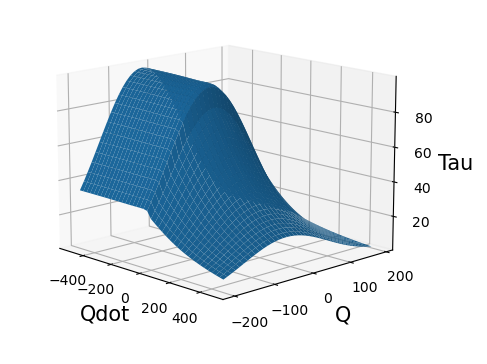
\includegraphics[width=\columnwidth]{figures/graph_force_vitesse_longueur.png}\\
\caption{Surface representing the nonlinear constraint for torque/position/velocity \comment{relationship}{which joint ?}}
\label{fig:graph_force_vitesse_longueur}
\end{figure}